%&preformat-disser
\RequirePackage[l2tabu,orthodox]{nag} % Раскомментировав, можно в логе получать рекомендации относительно правильного использования пакетов и предупреждения об устаревших и нерекомендуемых пакетах
% Формат А4, 14pt (ГОСТ Р 7.0.11-2011, 5.3.6)
\documentclass[a4paper,14pt,oneside,openany]{memoir}

%%%%%%%%%%%%%%%%%%%%%%%%%%%%%%%%%%%%%%%%%%%%%%%%%%%%%%%%%%%%%%%%%%%%%%%%%%%%%%%%
%%%% Файл упрощённых настроек шаблона, общих для диссертации и автореферата %%%%
%%%%%%%%%%%%%%%%%%%%%%%%%%%%%%%%%%%%%%%%%%%%%%%%%%%%%%%%%%%%%%%%%%%%%%%%%%%%%%%%

%%% Режим черновика %%%
\makeatletter
\@ifundefined{c@draft}{
  \newcounter{draft}
  \setcounter{draft}{0}  % 0 --- чистовик (максимальное соблюдение ГОСТ)
                         % 1 --- черновик (отклонения от ГОСТ, но быстрая
                         %       сборка итоговых PDF)
}{}
\makeatother

%%% Пометки в тексте %%%
\makeatletter
\@ifundefined{c@showmarkup}{
  \newcounter{showmarkup}
  \setcounter{showmarkup}{0}  % 0 --- скрыть пометки
                              % 1 --- показывать пометки
}{}
\makeatother

%%% Использование в pdflatex шрифтов не по-умолчанию %%%
\makeatletter
\@ifundefined{c@usealtfont}{
  \newcounter{usealtfont}
  \setcounter{usealtfont}{1}    % 0 --- шрифты на базе Computer Modern
                                % 1 --- использовать пакет pscyr, при его
                                %       наличии
                                % 2 --- использовать пакет XCharter, при наличии
                                %       подходящей версии
}{}
\makeatother

%%% Использование в xelatex и lualatex семейств шрифтов %%%
\makeatletter
\@ifundefined{c@fontfamily}{
  \newcounter{fontfamily}
  \setcounter{fontfamily}{1}  % 0 --- CMU семейство. Используется как fallback;
                              % 1 --- Шрифты от MS (Times New Roman и компания)
                              % 2 --- Семейство Liberation
}{}
\makeatother

%%% Библиография %%%
\makeatletter
\@ifundefined{c@bibliosel}{
  \newcounter{bibliosel}
  \setcounter{bibliosel}{0}   % 0 --- встроенная реализация с загрузкой файла
                              %       через движок bibtex8;
                              % 1 --- реализация пакетом biblatex через движок
                              %       biber
}{}
\makeatother

%%% Вывод типов ссылок в библиографии %%%
\makeatletter
\@ifundefined{c@mediadisplay}{
  \newcounter{mediadisplay}
  \setcounter{mediadisplay}{1}   % 0 --- не делать ничего; надписи [Текст] и
                                 %       [Эл. ресурс] будут выводиться только в ссылках с
                                 %       заполненным полем `media`;
                                 % 1 --- автоматически добавлять надпись [Текст] к ссылкам с
                                 %       незаполненным полем `media`; таким образом, у всех
                                 %       источников будет указан тип, что соответствует
                                 %       требованиям ГОСТ
                                 % 2 --- автоматически удалять надписи [Текст], [Эл. Ресурс] и др.;
                                 %       не соответствует ГОСТ
                                 % 3 --- автоматически удалять надпись [Текст];
                                 %       не соответствует ГОСТ
                                 % 4 --- автоматически удалять надпись [Эл. Ресурс];
                                 %       не соответствует ГОСТ
}{}
\makeatother

%%% Предкомпиляция tikz рисунков для ускорения работы %%%
\makeatletter
\@ifundefined{c@imgprecompile}{
  \newcounter{imgprecompile}
  \setcounter{imgprecompile}{0}   % 0 --- без предкомпиляции;
                                  % 1 --- пользоваться предварительно
                                  %       скомпилированными pdf вместо генерации
                                  %       заново из tikz
}{}
\makeatother
            % общие настройки шаблона
\input{common/packages}         % Пакеты общие для диссертации и автореферата
\usepackage{pdflscape}
\synopsisfalse                      % Этот документ --- не автореферат
\input{Dissertation/dispackages}    % Пакеты для диссертации
\input{Dissertation/userpackages}   % Пакеты для специфических пользовательских задач

%%%%%%%%%%%%%%%%%%%%%%%%%%%%%%%%%%%%%%%%%%%%%%%%%%%%%%%%%%%%%%%%%%%%%%%%%%%%%%%%
%%%% Файл упрощённых настроек шаблона, общих для диссертации и автореферата %%%%
%%%%%%%%%%%%%%%%%%%%%%%%%%%%%%%%%%%%%%%%%%%%%%%%%%%%%%%%%%%%%%%%%%%%%%%%%%%%%%%%

%%% Режим черновика %%%
\makeatletter
\@ifundefined{c@draft}{
  \newcounter{draft}
  \setcounter{draft}{0}  % 0 --- чистовик (максимальное соблюдение ГОСТ)
                         % 1 --- черновик (отклонения от ГОСТ, но быстрая
                         %       сборка итоговых PDF)
}{}
\makeatother

%%% Пометки в тексте %%%
\makeatletter
\@ifundefined{c@showmarkup}{
  \newcounter{showmarkup}
  \setcounter{showmarkup}{0}  % 0 --- скрыть пометки
                              % 1 --- показывать пометки
}{}
\makeatother

%%% Использование в pdflatex шрифтов не по-умолчанию %%%
\makeatletter
\@ifundefined{c@usealtfont}{
  \newcounter{usealtfont}
  \setcounter{usealtfont}{1}    % 0 --- шрифты на базе Computer Modern
                                % 1 --- использовать пакет pscyr, при его
                                %       наличии
                                % 2 --- использовать пакет XCharter, при наличии
                                %       подходящей версии
}{}
\makeatother

%%% Использование в xelatex и lualatex семейств шрифтов %%%
\makeatletter
\@ifundefined{c@fontfamily}{
  \newcounter{fontfamily}
  \setcounter{fontfamily}{1}  % 0 --- CMU семейство. Используется как fallback;
                              % 1 --- Шрифты от MS (Times New Roman и компания)
                              % 2 --- Семейство Liberation
}{}
\makeatother

%%% Библиография %%%
\makeatletter
\@ifundefined{c@bibliosel}{
  \newcounter{bibliosel}
  \setcounter{bibliosel}{0}   % 0 --- встроенная реализация с загрузкой файла
                              %       через движок bibtex8;
                              % 1 --- реализация пакетом biblatex через движок
                              %       biber
}{}
\makeatother

%%% Вывод типов ссылок в библиографии %%%
\makeatletter
\@ifundefined{c@mediadisplay}{
  \newcounter{mediadisplay}
  \setcounter{mediadisplay}{1}   % 0 --- не делать ничего; надписи [Текст] и
                                 %       [Эл. ресурс] будут выводиться только в ссылках с
                                 %       заполненным полем `media`;
                                 % 1 --- автоматически добавлять надпись [Текст] к ссылкам с
                                 %       незаполненным полем `media`; таким образом, у всех
                                 %       источников будет указан тип, что соответствует
                                 %       требованиям ГОСТ
                                 % 2 --- автоматически удалять надписи [Текст], [Эл. Ресурс] и др.;
                                 %       не соответствует ГОСТ
                                 % 3 --- автоматически удалять надпись [Текст];
                                 %       не соответствует ГОСТ
                                 % 4 --- автоматически удалять надпись [Эл. Ресурс];
                                 %       не соответствует ГОСТ
}{}
\makeatother

%%% Предкомпиляция tikz рисунков для ускорения работы %%%
\makeatletter
\@ifundefined{c@imgprecompile}{
  \newcounter{imgprecompile}
  \setcounter{imgprecompile}{0}   % 0 --- без предкомпиляции;
                                  % 1 --- пользоваться предварительно
                                  %       скомпилированными pdf вместо генерации
                                  %       заново из tikz
}{}
\makeatother
      % Упрощённые настройки шаблона

\input{common/newnames}         % Новые переменные, для всего проекта

%%% Основные сведения %%%
\newcommand{\thesisAuthorLastName}{Самойлов}
\newcommand{\thesisAuthorOtherNames}{Илья Сергеевич}
\newcommand{\thesisAuthorInitials}{И.\,С.}
\newcommand{\thesisAuthor}             % Диссертация, ФИО автора
{%
    \texorpdfstring{% \texorpdfstring takes two arguments and uses the first for (La)TeX and the second for pdf
        \thesisAuthorLastName~\thesisAuthorOtherNames% так будет отображаться на титульном листе или в тексте, где будет использоваться переменная
    }{%
        \thesisAuthorLastName, \thesisAuthorOtherNames% эта запись для свойств pdf-файла. В таком виде, если pdf будет обработан программами для сбора библиографических сведений, будет правильно представлена фамилия.
    }
}
\newcommand{\thesisAuthorShort}        % Диссертация, ФИО автора инициалами
{\thesisAuthorInitials~\thesisAuthorLastName}
%\newcommand{\thesisUdk}                % Диссертация, УДК
%{\fixme{xxx.xxx}}
\newcommand{\thesisTitle}              % Диссертация, название
{Исследование электронной структуры $\beta$-дикетонатов дифторидов бора
 и их азотсодержащих аналогов методами квантовой химии, оптической и фотоэлектронной спектроскопии}
\newcommand{\thesisSpecialtyNumber}    % Диссертация, специальность, номер
{01.04.05}
\newcommand{\thesisSpecialtyTitle}     % Диссертация, специальность, название (название взято с сайта ВАК для примера)
{Оптика}
%% \newcommand{\thesisSpecialtyTwoNumber} % Диссертация, вторая специальность, номер
%% {\fixme{XX.XX.XX}}
%% \newcommand{\thesisSpecialtyTwoTitle}  % Диссертация, вторая специальность, название
%% {\fixme{Теория и~методика физического воспитания, спортивной тренировки,
%% оздоровительной и~адаптивной физической культуры}}
\newcommand{\thesisDegree}             % Диссертация, ученая степень
{кандидата физико-математических наук}
\newcommand{\thesisDegreeShort}        % Диссертация, ученая степень, краткая запись
{\fixme{канд. физ.-мат. наук}}
\newcommand{\thesisCity}               % Диссертация, город написания диссертации
{Санкт-Петербург}
\newcommand{\thesisYear}               % Диссертация, год написания диссертации
{\the\year}
\newcommand{\thesisOrganization}       % Диссертация, организация
{Федеральное государственное бюджетное образовательное учреждение высшего профессионального образования\\
 <<Санкт-Петербургский государственный университет>>}
\newcommand{\thesisOrganizationShort}  % Диссертация, краткое название организации для доклада
{\fixme{СПбГУ}}

\newcommand{\thesisInOrganization}     % Диссертация, организация в предложном падеже: Работа выполнена в ...
{\fixme{учреждении с~длинным длинным длинным длинным названием, в~котором
выполнялась данная диссертационная работа}}

%% \newcommand{\supervisorDead}{}           % Рисовать рамку вокруг фамилии
\newcommand{\supervisorFio}              % Научный руководитель, ФИО
{Чижов Юрий Владимирович}
\newcommand{\supervisorRegalia}          % Научный руководитель, регалии
{д-р физ.-мат. наук, профессор}
\newcommand{\supervisorFioShort}         % Научный руководитель, ФИО
{Ю.\,В.~Чижов}
\newcommand{\supervisorRegaliaShort}     % Научный руководитель, регалии
{д-р физ.-мат. наук,~профессор}

%% \newcommand{\supervisorTwoDead}{}        % Рисовать рамку вокруг фамилии
 \newcommand{\supervisorTwoFio}           % Второй научный руководитель, ФИО
 {Тихонов Сергей Александрович}
 \newcommand{\supervisorTwoRegalia}       % Второй научный руководитель, регалии
 {канд. физ.-мат. наук}
 \newcommand{\supervisorTwoFioShort}      % Второй научный руководитель, ФИО
 {С.\,А.~Тихонов}
 \newcommand{\supervisorTwoRegaliaShort}  % Второй научный руководитель, регалии
 {канд. физ.-мат. наук}

\newcommand{\opponentOneFio}           % Оппонент 1, ФИО
{\fixme{Фамилия Имя Отчество}}
\newcommand{\opponentOneRegalia}       % Оппонент 1, регалии
{\fixme{доктор физико-математических наук, профессор}}
\newcommand{\opponentOneJobPlace}      % Оппонент 1, место работы
{\fixme{Не очень длинное название для места работы}}
\newcommand{\opponentOneJobPost}       % Оппонент 1, должность
{\fixme{старший научный сотрудник}}

\newcommand{\opponentTwoFio}           % Оппонент 2, ФИО
{\fixme{Фамилия Имя Отчество}}
\newcommand{\opponentTwoRegalia}       % Оппонент 2, регалии
{\fixme{кандидат физико-математических наук}}
\newcommand{\opponentTwoJobPlace}      % Оппонент 2, место работы
{\fixme{Основное место работы c длинным длинным длинным длинным названием}}
\newcommand{\opponentTwoJobPost}       % Оппонент 2, должность
{\fixme{старший научный сотрудник}}

%% \newcommand{\opponentThreeFio}         % Оппонент 3, ФИО
%% {\fixme{Фамилия Имя Отчество}}
%% \newcommand{\opponentThreeRegalia}     % Оппонент 3, регалии
%% {\fixme{кандидат физико-математических наук}}
%% \newcommand{\opponentThreeJobPlace}    % Оппонент 3, место работы
%% {\fixme{Основное место работы c длинным длинным длинным длинным названием}}
%% \newcommand{\opponentThreeJobPost}     % Оппонент 3, должность
%% {\fixme{старший научный сотрудник}}

\newcommand{\leadingOrganizationTitle} % Ведущая организация, дополнительные строки. Удалить, чтобы не отображать в автореферате
{Федеральное государственное бюджетное образовательное учреждение высшего
профессионального образования с~длинным длинным длинным длинным названием}

\newcommand{\defenseDate}              % Защита, дата
{\fixme{DD mmmmmmmm YYYY~г.~в~XX часов}}
\newcommand{\defenseCouncilNumber}     % Защита, номер диссертационного совета
{\fixme{Д\,123.456.78}}
\newcommand{\defenseCouncilTitle}      % Защита, учреждение диссертационного совета
{\fixme{Название учреждения}}
\newcommand{\defenseCouncilAddress}    % Защита, адрес учреждение диссертационного совета
{\fixme{Адрес}}
\newcommand{\defenseCouncilPhone}      % Телефон для справок
{\fixme{+7~(0000)~00-00-00}}

\newcommand{\defenseSecretaryFio}      % Секретарь диссертационного совета, ФИО
{\fixme{Фамилия Имя Отчество}}
\newcommand{\defenseSecretaryRegalia}  % Секретарь диссертационного совета, регалии
{\fixme{д-р~физ.-мат. наук}}            % Для сокращений есть ГОСТы, например: ГОСТ Р 7.0.12-2011 + http://base.garant.ru/179724/#block_30000

\newcommand{\synopsisLibrary}          % Автореферат, название библиотеки
{\fixme{Название библиотеки}}
\newcommand{\synopsisDate}             % Автореферат, дата рассылки
{\fixme{DD mmmmmmmm}\the\year~года}

% To avoid conflict with beamer class use \providecommand
\providecommand{\keywords}%            % Ключевые слова для метаданных PDF диссертации и автореферата
{}
             % Основные сведения
\input{common/fonts}            % Определение шрифтов (частичное)
\input{common/styles}           % Стили общие для диссертации и автореферата
\input{Dissertation/disstyles}  % Стили для диссертации
\input{Dissertation/userstyles} % Стили для специфических пользовательских задач

%%% Библиография. Выбор движка для реализации %%%
% Здесь только проверка установленного ключа. Сама настройка выбора движка
% размещена в common/setup.tex
\ifnumequal{\value{bibliosel}}{0}{%
    \input{biblio/predefined}   % Встроенная реализация с загрузкой файла через движок bibtex8
}{
    \input{biblio/biblatex}     % Реализация пакетом biblatex через движок biber
}

% Вывести информацию о выбранных опциях в лог сборки
\typeout{Selected options:}
\typeout{Draft mode: \arabic{draft}}
\typeout{Font: \arabic{fontfamily}}
\typeout{AltFont: \arabic{usealtfont}}
\typeout{Bibliography backend: \arabic{bibliosel}}
\typeout{Precompile images: \arabic{imgprecompile}}
% Вывести информацию о версиях используемых библиотек в лог сборки
\listfiles

%%% Управление компиляцией отдельных частей диссертации %%%
% Необходимо сначала иметь полностью скомпилированный документ, чтобы все
% промежуточные файлы были в наличии
% Затем, для вывода отдельных частей можно воспользоваться командой \includeonly
% Ниже примеры использования команды:
%
%\includeonly{Dissertation/part2}
%\includeonly{Dissertation/contents,Dissertation/appendix,Dissertation/conclusion}
%
% Если все команды закомментированы, то документ будет выведен в PDF файл полностью

\begin{document}
%%% Переопределение именований типовых разделов
% https://tex.stackexchange.com/a/156050
\gappto\captionsrussian{\input{common/renames}\unskip} % for polyglossia and babel
\input{common/renames}

%%% Структура диссертации (ГОСТ Р 7.0.11-2011, 4)
% Титульный лист (ГОСТ Р 7.0.11-2001, 5.1)
\thispagestyle{empty}
\begin{center}
\thesisOrganization
\end{center}
%
\vspace{0pt plus4fill} %число перед fill = кратность относительно некоторого расстояния fill, кусками которого заполнены пустые места
\IfFileExists{images/logo.pdf}{
  \begin{minipage}[b]{0.5\linewidth}
    \begin{flushleft}
      
\includegraphics[height=3.5cm]{logo}
    \end{flushleft}
  \end{minipage}%
  \begin{minipage}[b]{0.5\linewidth}
    \begin{flushright}
      
\includegraphics[height=2.5cm]{sign}\\
      На правах рукописи\\
%      \textsl {УДК \thesisUdk}
    \end{flushright}
  \end{minipage}
}{
\begin{flushright}
На правах рукописи

%\textsl {УДК \thesisUdk}
\end{flushright}
}
%
\vspace{0pt plus6fill} %число перед fill = кратность относительно некоторого расстояния fill, кусками которого заполнены пустые места
\begin{center}
{\large \thesisAuthor}
\end{center}
%
\vspace{0pt plus1fill} %число перед fill = кратность относительно некоторого расстояния fill, кусками которого заполнены пустые места
\begin{center}
\textbf {\large %\MakeUppercase
\thesisTitle}

\vspace{0pt plus2fill} %число перед fill = кратность относительно некоторого расстояния fill, кусками которого заполнены пустые места
{%\small
Специальность \thesisSpecialtyNumber\ "---

<<\thesisSpecialtyTitle>>
}

\ifdefined\thesisSpecialtyTwoNumber
{%\small
Специальность \thesisSpecialtyTwoNumber\ "---

<<\thesisSpecialtyTwoTitle>>
}
\fi

\vspace{0pt plus2fill} %число перед fill = кратность относительно некоторого расстояния fill, кусками которого заполнены пустые места
Диссертация на соискание учёной степени

\thesisDegree
\end{center}
%
\vspace{0pt plus3fill} %число перед fill = кратность относительно некоторого расстояния fill, кусками которого заполнены пустые места
\begin{flushright}
\ifdefined\supervisorTwoFio
Научный руководитель:

\supervisorRegalia

\ifdefined\supervisorDead
\framebox{\supervisorFio}
\else
\supervisorFio\\
\fi
\vspace{0pt plus2fill}
Научный консультант:\\
\supervisorTwoRegalia

\ifdefined\supervisorTwoDead
\framebox{\supervisorTwoFio}
\else
\supervisorTwoFio
\fi
\else
Научный руководитель:

\supervisorRegalia

\ifdefined\supervisorDead
\framebox{\supervisorFio}
\else
\supervisorFio
\fi
\fi

\end{flushright}
%
\vspace{0pt plus4fill} %число перед fill = кратность относительно некоторого расстояния fill, кусками которого заполнены пустые места
{\centering\thesisCity\ "--- \thesisYear\par}
           % Титульный лист
\include{Dissertation/contents}        % Оглавление
\printnomenclature[3.5cm] % Значение ширины столбца с обозначениями стоит подбирать вручную

\newpage

\begin{figure}[ht]
    \caption{Исследованные соединения I-X}
    \centerfloat{
        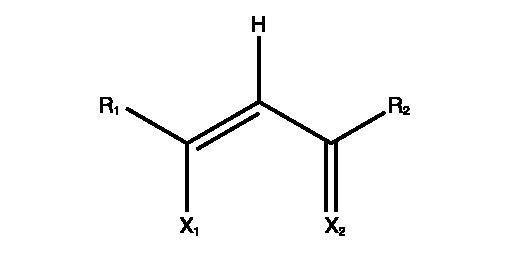
\includegraphics[scale=1.25]{1_stroenie-beta.pdf}
    }
\label{RIS1}
\end{figure}

\begin{table} [htbp]%
    \centering
    \caption{Исследованные соединения}%
    \label{tab:comopund_list_1}% 
    \renewcommand{\arraystretch}{1.5}%% Увеличение расстояния между рядами, для улучшения восприятия.
    \begin{SingleSpace}
        \begin{tabular}{@{}@{\extracolsep{20pt}}llllll@{}} %Вертикальные полосы не используются принципиально, как и лишние горизонтальные (допускается по ГОСТ 2.105 пункт 4.4.5) % @{} позволяет прижиматься к краям
            \toprule     %%% верхняя линейка
            №         & Compound        & X$_1$      & X$_2$  & R$_1$      & R$_2$      \\
            \midrule 
            I.        & Hmal            & H          & O      & H          & H          \\
            II.       & Hacac           & H          & O      & CH$_3$     & CH$_3$     \\
            III.      & EnAcac          & NH$_2$     & O      & CH$_3$     & CH$_3$     \\
            IV.       & EnMeAcac        & NHCH$_3$   & O      & CH$_3$     & CH$_3$     \\
            V.        & CH$_3$SAcac     & SCH$_3$    & O      & CH$_3$     & CH$_3$     \\
            VI.       & HSHAc           & SH         & O      & CH$_3$     & CH$_3$     \\
            VII.      & SOHAc           & OH         & S      & CH$_3$     & CH$_3$     \\
            VIII.     & HtFAc           & OH         & O      & CF$_3$     & CH$_3$     \\
            IX.       & HhFAc           & OH         & O      & CF$_3$     & CF$_3$     \\
            \bottomrule 
        \end{tabular}
    \end{SingleSpace}
\end{table}

\newpage

\begin{figure}[ht]
    \centerfloat{
        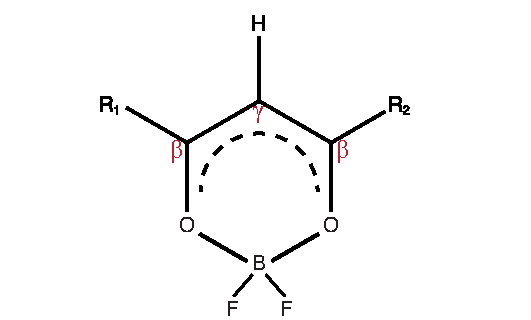
\includegraphics[scale=1.25]{2_stroenie_boron.pdf}
    }
\label{fig:latex}
\end{figure}

\begin{table} [htbp]%
    \centering
    \caption{Исследованные соединения Часть 2}%
    \label{tab:comopund_list_2}% 
    \renewcommand{\arraystretch}{1.5}%% Увеличение расстояния между рядами, для улучшения восприятия.
    \begin{SingleSpace}
        \begin{tabular}{@{}@{\extracolsep{20pt}}llll@{}} %Вертикальные полосы не используются принципиально, как и лишние горизонтальные (допускается по ГОСТ 2.105 пункт 4.4.5) % @{} позволяет прижиматься к краям
            \toprule     %%% верхняя линейка
            №      &Compound         & R$_1$      & R$_2$                           \\
            \midrule
            X.     & BF$_2$Acac      & CH$_3$     & CH$_3$                          \\
            XI.    & BF$_2$bac       & CH$_3$     & C$_6$H$_5$                      \\
            XII.   & BF$_2$tac       & CH$_3$     & 4$-$CH$_3$C$_6$H$_4$            \\
            XIII.  & BF$_2$xac       & CH$_3$     & 2,4$-($CH$_3$)$_2$C$_6$H$_3$    \\
            XIV.   &                 & CH$_3$     & 4$-$biphenyl                    \\
            XV.    &                 & CH$_3$     & 4$-$fluorenyl                   \\
            XVI.   &                 & CH$_3$     & 4$-$trans$-$stilbene            \\
            XVII.  & BF$_2$Dbm       & C$_6$H$_5$ & C$_6$H$_5$                      \\
            XVIII. & BF$_2$anth      & CH$_3$     & C$_{14}$H$_9$                   \\
            XIX.   & BF$_2$naph      & CH$_3$     & C$_{10}$H$_7$                   \\
            XX.    & BF$_2$ben       & CH$_3$     & CO$_2$C$_6$H$_4$                \\
            \bottomrule 
        \end{tabular}
    \end{SingleSpace}
\end{table}        % Список сокращений и условных обозначений
%\ifnumequal{\value{contnumfig}}{1}{}{\counterwithout{figure}{chapter}}
%\ifnumequal{\value{contnumtab}}{1}{}{\counterwithout{table}{chapter}}
\chapter*{Введение}                         % Заголовок
\addcontentsline{toc}{chapter}{Введение}    % Добавляем его в оглавление

Среди координационных соединений особое внимание  привлекают $\beta-$дикетонаты дифторида бора, обладающие
интенсивной люминесценцией  \cite{butler2016mechanochromic,fedorenko2017new,zhang2018reversible,
guieu2015synthesis,wang2015red,mamiya2016photochemically}, способностью к формированию эксимеров 
\cite{mirochnik2003crystal,bukvetskii2010crystal} и эксиплексов \cite{chow1995exciplexes,chow1995exciplex},
люминесцентным термохромизмом \cite{mirocnik2005obratimyj} и жидкокристаллическим полиморфизмом 
\cite{turanova2010liquid,mayoral2011alkoxy,sanchez2012liquid,giziroglu20141}. $\beta-$Дикетонаты дифторида бора
находят применение в качестве лазерных красителей \cite{czerney1990german}, органических светодиодов 
\cite{derosa2015tailoring,daly2016blue} , оптических хемосенсоров \cite{zhai2016nanofibers,fraser2018oxygen,
samonina2015luminescent}, активных компонентов солнечных коллекторов \cite{halik2003german}, материалов для 
нелинейной оптики \cite{kammler1996second} и полимерных оптических материалов\cite{tanaka2013facile,
zhang2009role}.
Установление взаимосвязей электронного строения и спектральных характеристик $\beta-$дикетонатов дифторида бора 
открывает возможности для создания новых оптических материалов на их основе. Поэтому моделирование электронной 
структуры и интерпретация фотоэлектронных и абсорбционных спектров $\beta-$дикетонатов дифторида бора является 
актуальной задачей.

Люминесцентные свойства $\beta-$дикетонатов дифторида бора определяются природой заместителей в $\beta-$положениях
(\ref{RIS1}). Замещение в $\gamma-$положении перспективно для формирования комплексов, обладающих химическими 
свойствами необходимыми для иммобилизации на поверхности или внедрения в другие структуры. Кроме того, введение
$\gamma-$заместителя должно препятствовать свободному вращению ароматических групп в $\beta-$положениях, что 
может привести к батохромному сдвигу спектра люминесценции и увеличению квантового выхода.
В настоящий момент практически отсутствуют сведения о влиянии заместителей в $\gamma-$положении на оптические 
свойства $\beta-$дикетонатов дифторида бора \cite{svistunova2008alpha,tikhonov2018electronic}.
Поэтому заслуживает внимания изучение электронного строения $\gamma-$замещённых ацетилацетонатов дифторида бора 
$-$ простейших $\beta-$дикетонатов дифторида бора с функциональными группами в $\gamma-$положении.
Наиболее достоверную информацию об электронном строении химических соединений можно получить при совместном 
применении методов фотоэлектронной спектроскопии и квантовой химии \cite{nefedov1987elektronnaa,
nefedov1989elektronnaa,osmushko2016application}.
Применение метода абсорбционной спектроскопии и результатов моделирования возбуждённых состояний позволяет
устанавливать взаимосвязи молекулярной структуры и оптических свойств хелатов бора на основе анализа электронных
эффектов замещения \cite{karasev2006fotofizika,kazachek2015excited,margar2016fluorescent},а также давать
рекомендации для синтеза новых комплексов с заданными положениями максимумов спектра флюоресценции
\cite{ponce2018searching}.\\


\newcommand{\actuality}{}
\newcommand{\progress}{}
\newcommand{\aim}{{\textbf\aimTXT}}
\newcommand{\tasks}{\textbf{\tasksTXT}}
\newcommand{\novelty}{\textbf{\noveltyTXT}}
\newcommand{\influence}{\textbf{\influenceTXT}}
\newcommand{\methods}{\textbf{\methodsTXT}}
\newcommand{\defpositions}{\textbf{\defpositionsTXT}}
\newcommand{\reliability}{\textbf{\reliabilityTXT}}
\newcommand{\probation}{\textbf{\probationTXT}}
\newcommand{\contribution}{\textbf{\contributionTXT}}
\newcommand{\publications}{\textbf{\publicationsTXT}}

\input{common/characteristic} % Характеристика работы по структуре во введении и в автореферате не отличается (ГОСТ Р 7.0.11, пункты 5.3.1 и 9.2.1), потому её загружаем из одного и того же внешнего файла, предварительно задав форму выделения некоторым параметрам

\textbf{Объем и структура работы.} Диссертация состоит из~введения,
\formbytotal{totalchapter}{глав}{ы}{}{},
заключения и
\formbytotal{totalappendix}{приложен}{ия}{ий}{}.
%% на случай ошибок оставляю исходный кусок на месте, закомментированным
%Полный объём диссертации составляет  \ref*{TotPages}~страницу
%с~\totalfigures{}~рисунками и~\totaltables{}~таблицами. Список литературы
%содержит \total{citenum}~наименований.
%
Полный объём диссертации составляет
\formbytotal{TotPages}{страниц}{у}{ы}{}, включая
\formbytotal{totalcount@figure}{рисун}{ок}{ка}{ков} и
\formbytotal{totalcount@table}{таблиц}{у}{ы}{}.
Список литературы содержит
\formbytotal{citenum}{наименован}{ие}{ия}{ий}.

\begin{landscape}
\begin{figure}[ht]
    \centerfloat{
    \includegraphics[scale=0.75]{I-IItest.pdf}
    }
\label{spektr}
\caption{ Бенчмарк выаоывао товыат оывта оывтао тывоа тоыта оытвоа тыво атыолвта оывта олывта оыта отыво 
Исследованные соединения I-II}
\end{figure}
\end{landscape}    % Введение
%\ifnumequal{\value{contnumfig}}{1}{\counterwithout{figure}{chapter}
%}{\counterwithin{figure}{chapter}}
%\ifnumequal{\value{contnumtab}}{1}{\counterwithout{table}{chapter}
%}{\counterwithin{table}{chapter}}
%\chapter{Оформление различных элементов}\label{ch:ch1}

\section{Форматирование текста}\label{sec:ch1/sec1}           % Глава 1
%\chapter{Длинное название главы, в которой мы смотрим на~примеры того, как будут верстаться изображения и~списки}\label{ch:ch2}

\section{Одиночное изображение}\label{sec:ch2/sec1}

           % Глава 2
%\chapter{Вёрстка таблиц}\label{ch:ch3}

\section{Таблица обыкновенная}\label{sec:ch3/sect1}


\clearpage
           % Глава 3
%\include{Dissertation/conclusion}      % Заключение
%\include{Dissertation/dictionary}      % Словарь терминов
\include{Dissertation/references}      % Список литературы
%\include{Dissertation/lists}           % Списки таблиц и изображений (иллюстративный материал)

\setcounter{totalchapter}{\value{chapter}} % Подсчёт количества глав

%%% Настройки для приложений
\appendix
% Оформление заголовков приложений ближе к ГОСТ:
\setlength{\midchapskip}{20pt}
\renewcommand*{\afterchapternum}{\par\nobreak\vskip \midchapskip}
\renewcommand\thechapter{\Asbuk{chapter}} % Чтобы приложения русскими буквами нумеровались

%\include{Dissertation/appendix}        % Приложения

\setcounter{totalappendix}{\value{chapter}} % Подсчёт количества приложений

\end{document}
